\documentclass[crop,tikz,convert={outext=.svg,command=\unexpanded{pdf2svg \infile\space\outfile}},multi=false]{standalone}[2012/04/13]

\usepackage[utf8]{inputenc}
\usepackage{amsmath, amssymb}
\usepackage{pgfplots}

%-------------------------------------
% Tikz and pgf options & definitions
%-------------------------------------
\pgfplotsset{compat=1.15}
\pgfmathsetseed{1}

\usetikzlibrary{positioning}
\usetikzlibrary{shapes}
\usetikzlibrary{backgrounds, fit}
\usetikzlibrary{calc}
\usetikzlibrary{decorations.markings}
\usetikzlibrary{matrix}

\def\colorvector at (#1,#2,#3){
\coordinate (A) at (#1, #2);
\filldraw[draw=black,fill=test!!+] (A)++(0,0) rectangle ++(0.25,0.25) node (A0) {};
\filldraw[draw=black,fill=test!!+] (A)++(0.3,0) rectangle ++(0.25,0.25) node (A1) {};
\filldraw[draw=black,fill=test!!+] (A)++(0.6,0) rectangle ++(0.25,0.25) node (A2) {};
\node[right=of A2, xshift=-7.5ex, yshift=-0.75ex] {$\ldots$};
\filldraw[draw=black,fill=test!!+] (A)++(1.5,0) rectangle ++(0.25,0.25) node (A4) {};
\node[left=of A1, xshift=4.4ex, yshift=-0.75ex] (BEG\i) {$#3=[$};
\node[right=of A4, xshift=-8ex, yshift=-0.75ex] (END\i) {$]^{T}$};
}

\begin{document}
\tikzset{every loop/.style={min distance=10mm,looseness=10}}
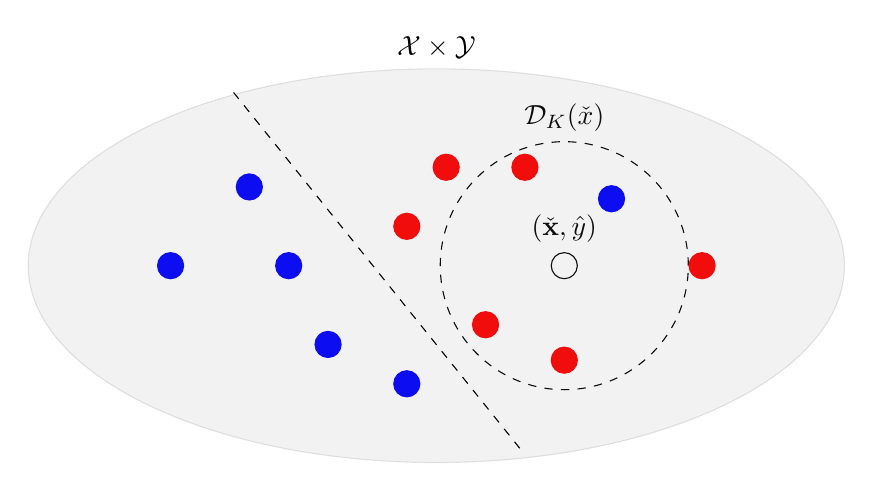
\begin{tikzpicture}
\node[draw, circle, minimum width =0.2 cm, color=blue, fill=blue] (x1) at (0, 0) {};
\node[draw, circle, minimum width =0.2 cm, color=blue, fill=blue] (x2) at (1, 1) {};
\node[draw, circle, minimum width =0.2 cm, color=blue, fill=blue] (x3) at (2, -1) {};
\node[draw, circle, minimum width =3.15 cm, color=black, dashed, fill=white, label=above:{${\cal D}_{K}(\check{x}) $}] (x5) at (5, 0) {};
\node[draw, circle, minimum width =0.2 cm, color=black, fill=white, label=above:{$ \left( \check{\bf x}, \hat{y} \right)$}] (x4) at (5, 0) {};
\node[draw, circle, minimum width =0.2 cm, color=blue, fill=blue] (x6) at (1.5, 0) {};
\node[draw, circle, minimum width =0.2 cm, color=blue, fill=blue] (x7) at (3, -1.5) {};
\node[draw, circle, minimum width =0.2 cm, color=red, fill=red] (x8) at (4.5, 1.25) {};
\node[draw, circle, minimum width =0.2 cm, color=red, fill=red] (x9) at (3, 0.5) {};
\node[draw, circle, minimum width =0.2 cm, color=blue, fill=blue] (x10) at (5.6, 0.85) {};
\node[draw, circle, minimum width =0.2 cm, color=red, fill=red] (x11) at (4, -0.75) {};
\node[draw, circle, minimum width =0.2 cm, color=red, fill=red] (x12) at (3.5, 1.25) {};
\node[draw, circle, minimum width =0.2 cm, color=red, fill=red] (x13) at (5, -1.2) {};
\node[draw, circle, minimum width =0.2 cm, color=red, fill=red] (x14) at (6.75, 0) {};
\node[fit={(x1)(x14)},draw, ellipse, fill=gray, opacity = 0.1, minimum width=3cm,minimum height=5cm,label=above:{${\cal X} \times {\cal Y} $}](X){};
\draw[dashed] (0.8,2.2) -- (4.5,-2.4);
\end{tikzpicture}
\end{document}